\begin{figure}[htbp]
	\centering
	\newcommand\sfMergeRealImag{0.85}
	\newcommand\gridnode[5]{
		\node (#1) at (#2 + #4 / 2,#3 + #5 / 2) [minimum width=#4cm * \sfMergeRealImag,minimum height=#5cm * \sfMergeRealImag] {};
		\draw[step=0.1] (#2 - 0.001,#3 - 0.001) grid (#2+#4 + 0.001,#3+#5 + 0.001);	
	}
	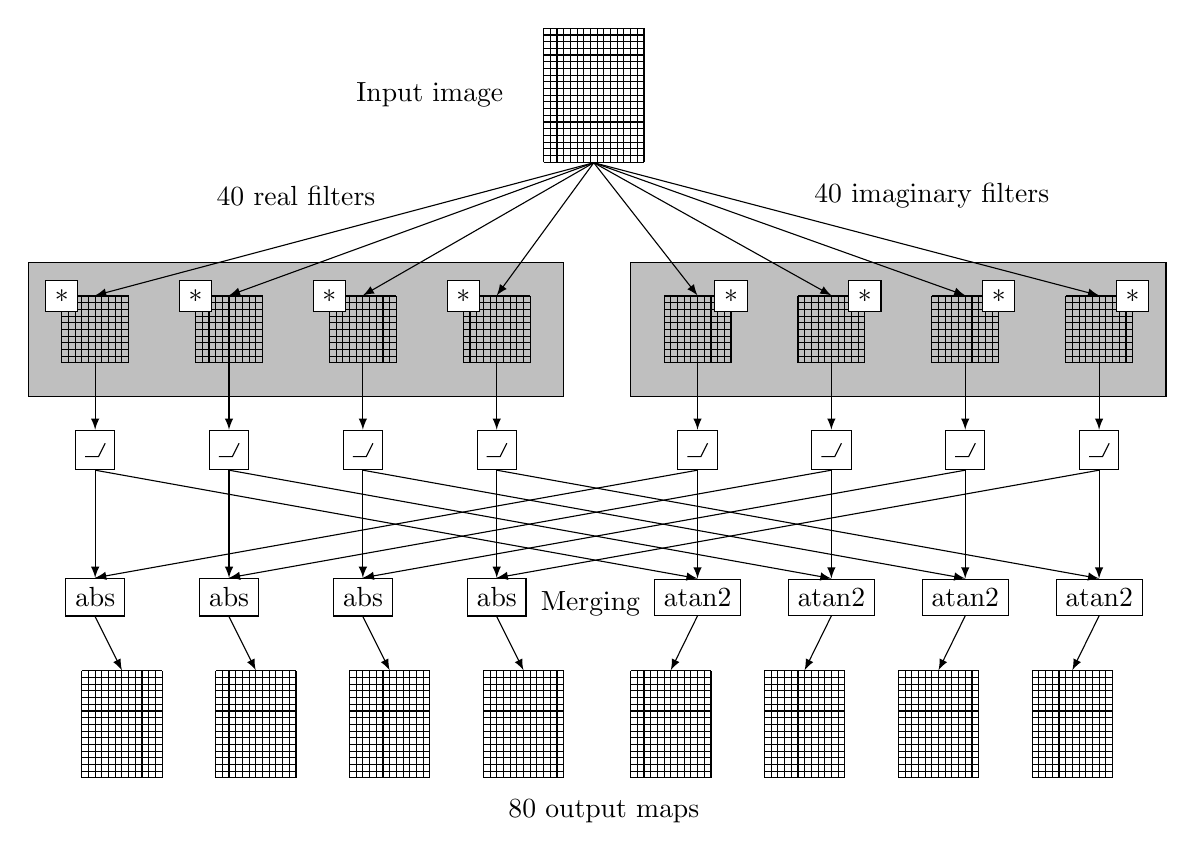
\begin{tikzpicture}[scale=\sfMergeRealImag,every path/.style={>=latex}]
		% draw input image
		\gridnode{inputimage}{7.7}{3}{1.5}{2}
	
		% draw background boxes
		\draw[fill=lightgray] (0,1.5) rectangle (8,-0.5);
		\draw[fill=lightgray] (9,1.5) rectangle (17,-0.5);
	
		% draw real filters
		\foreach \x in {0,...,3}
		{
			\gridnode{r\x}{\x * 2 + 0.5}{0}{1}{1}
			\node at (\x * 2 + .5, 1) [draw,fill=white] {$*$};
			\draw[->] (inputimage.south) to (r\x.north);
			\node (ar\x) at (\x * 2 + 1., -1.3) [draw,rectangle,minimum size=0.5cm] {};
			\draw[-] (\x * 2 + 0.85, -1.4) to (\x * 2 + 1.05,-1.4) to (\x * 2 + 1.15, -1.2);
			\draw[->] (r\x.south) to (ar\x.north);
		}
		
		% draw imaginary filters
		\foreach \x in {0,...,3}
		{
			\gridnode{i\x}{\x * 2 + 9.5}{0}{1}{1}
			\node at (\x * 2 + 10.5, 1) [draw,fill=white] {$*$};
			\draw[->] (inputimage.south) to (i\x.north);
			\node (ai\x) at (\x * 2 + 10., -1.3) [draw,rectangle,minimum size=0.5cm] {};
			\draw[-] (\x * 2 + 9.85, -1.4) to (\x * 2 + 10.05,-1.4) to (\x * 2 + 10.15, -1.2);
			\draw[->] (i\x.south) to (ai\x.north);
		}
		
		% draw abs operators
		\foreach \x in {0,...,3}
		{
			\node (abs\x) at (\x * 2 + 1,-3.5) [draw,rectangle] {abs};
			\draw[->] (ar\x.south) to (abs\x.north);
			\draw[->] (ai\x.south) to (abs\x.north);
		}
		
		% draw atan2 operators
		\foreach \x in {0,...,3}
		{
			\node (atan2\x) at (\x * 2 + 10,-3.5) [draw,rectangle] {atan2};
			\draw[->] (ar\x.south) to (atan2\x.north);
			\draw[->] (ai\x.south) to (atan2\x.north);
		}
		
		% draw abs output maps
		\foreach \x in {0,...,3}
		{
			\gridnode{o\x}{\x * 2 + 0.8}{-6.2}{1.2}{1.6}
			\draw[->] (abs\x.south) to (o\x.north);
		}
		
		% draw abs output maps
		\foreach \x in {0,...,3}
		{
			\gridnode{o\x}{\x * 2 + 9.}{-6.2}{1.2}{1.6}
			\draw[->] (atan2\x.south) to (o\x.north);
		}
		
		% draw text nodes
		\node at (6,4) {Input image};
		\node at (4,2.5) {40 real filters};
		\node at (13.5,2.5) {40 imaginary filters};
		\node at (8.4,-3.6) {Merging};
		\node at (8.6,-6.7) {80 output maps};
	\end{tikzpicture}
	\caption{A Gabor layer with both merging methods}
	\label{fig:merge_abs_atan2}
\end{figure}\
